\subsection{Grasper Verification}

\subsubsection{Holding Capacity} \label{sec:results:capacity}

Table \ref{tab:weight-inc} shows the weight increments added during the test,
the total weight at each step, and the result (OK or NOK based on whether the 
5-minute waiting period passed without the device breaking). The test ended without
failure being reached, because all available weights had been added.

This test gives a total verified holding capacity, after accounting for the 
electronics that were removed for the test, of 8.7 kg. The actual limit is still
unknown, due to the limited number of test weights available.

\begin{table}[H]
    \centering
    \caption{Weights of Grasper Components}
    \label{tab:weight-inc}
    \begin{tabular}{|c||c|c|c|}
        \hline
        Addition Number & Added Weight [g] & Total Weight [g] & Result\\
        \hline
        1 & 3830 & 3830 & OK\\
        2 & 1000 & 4830 & OK\\
        3 & 1000 & 5830 & OK\\
        4 & 1000 & 6830 & OK\\
        5 & 500 & 7330 & OK\\
        6 & 500 & 7830 & OK\\
        7 & 500 & 8330 & OK\\
        8 & 500 & 8830 & OK\\
        \hline
    \end{tabular}
\end{table}

\subsubsection{Weight}

\begin{table}[H]
    \centering
    \caption{Weights of Grasper Components}
    \label{tab:weights}
    \begin{tabular}{
        |>{\raggedright\arraybackslash}m{0.33\textwidth}|>{\raggedright\arraybackslash}m{0.33\textwidth}||
        >{\raggedright\arraybackslash}m{0.15\textwidth}|}
        \hline
        Component & Photo & Weight [g]\\
        \hline
        Base Plate and Clasp Mounts & 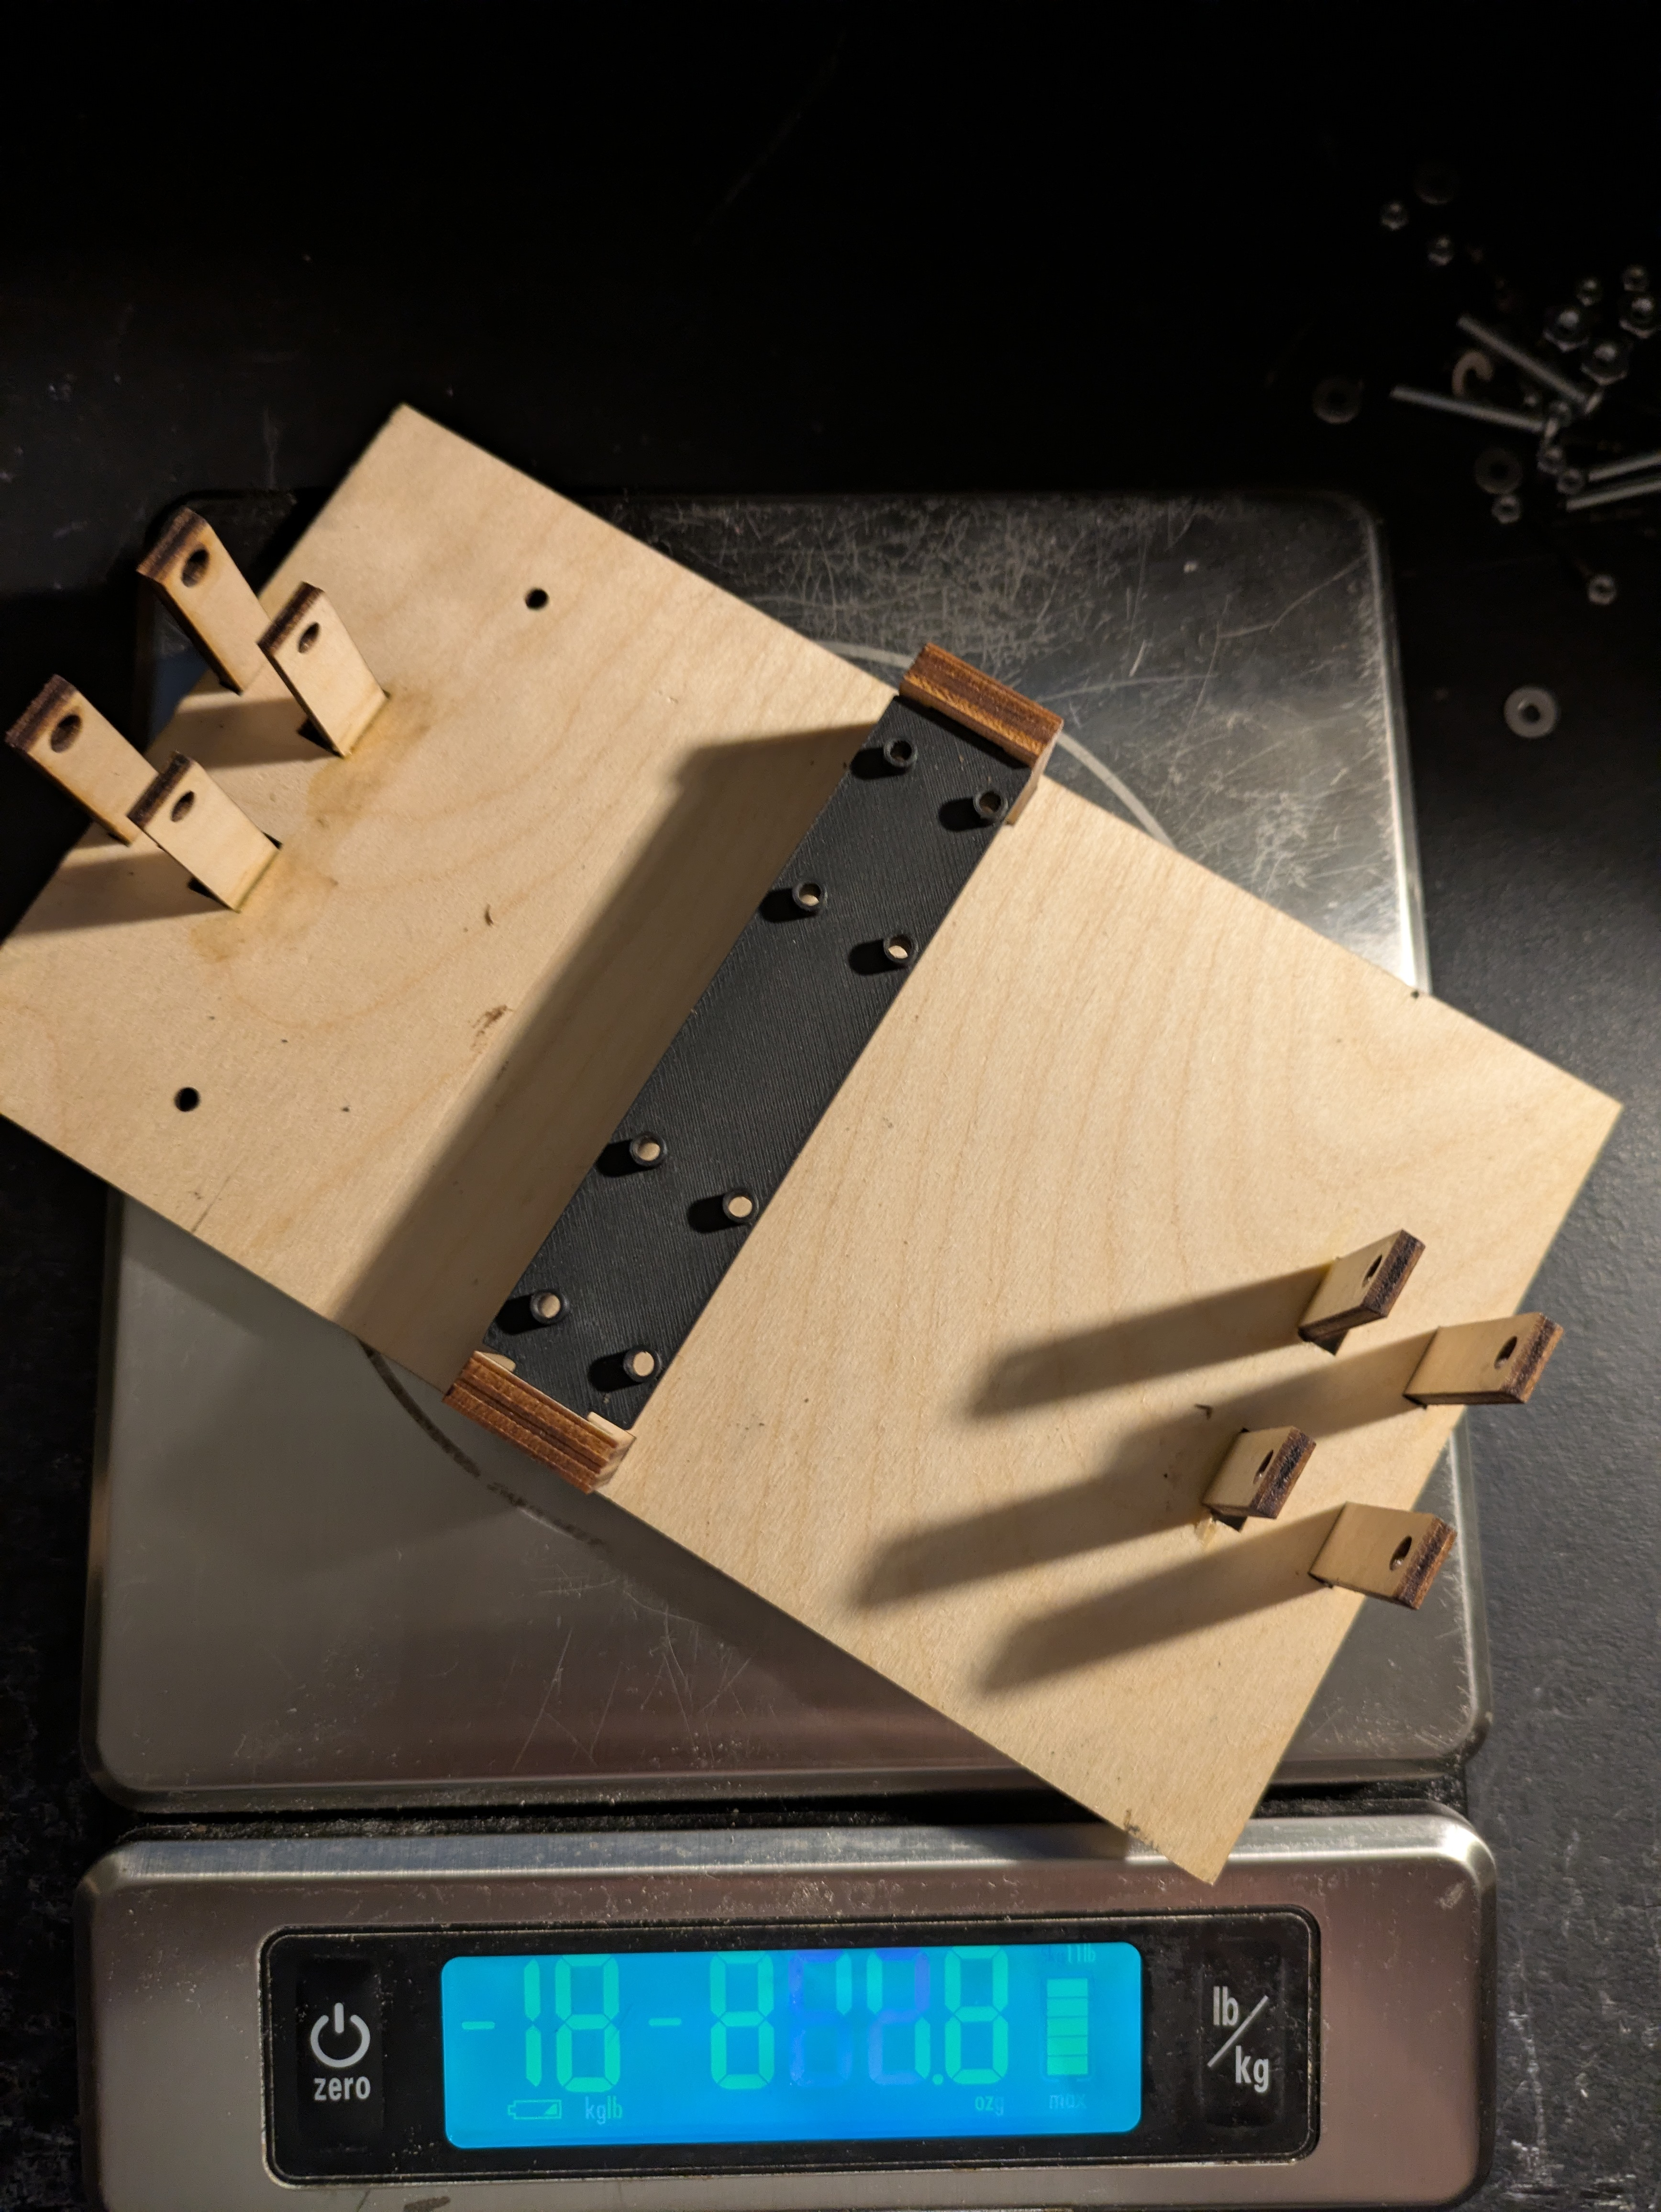
\includegraphics[width=0.2\textwidth]{sections/results/parts-base.jpg} & 62 \\
        Grasper (Average of Both) & 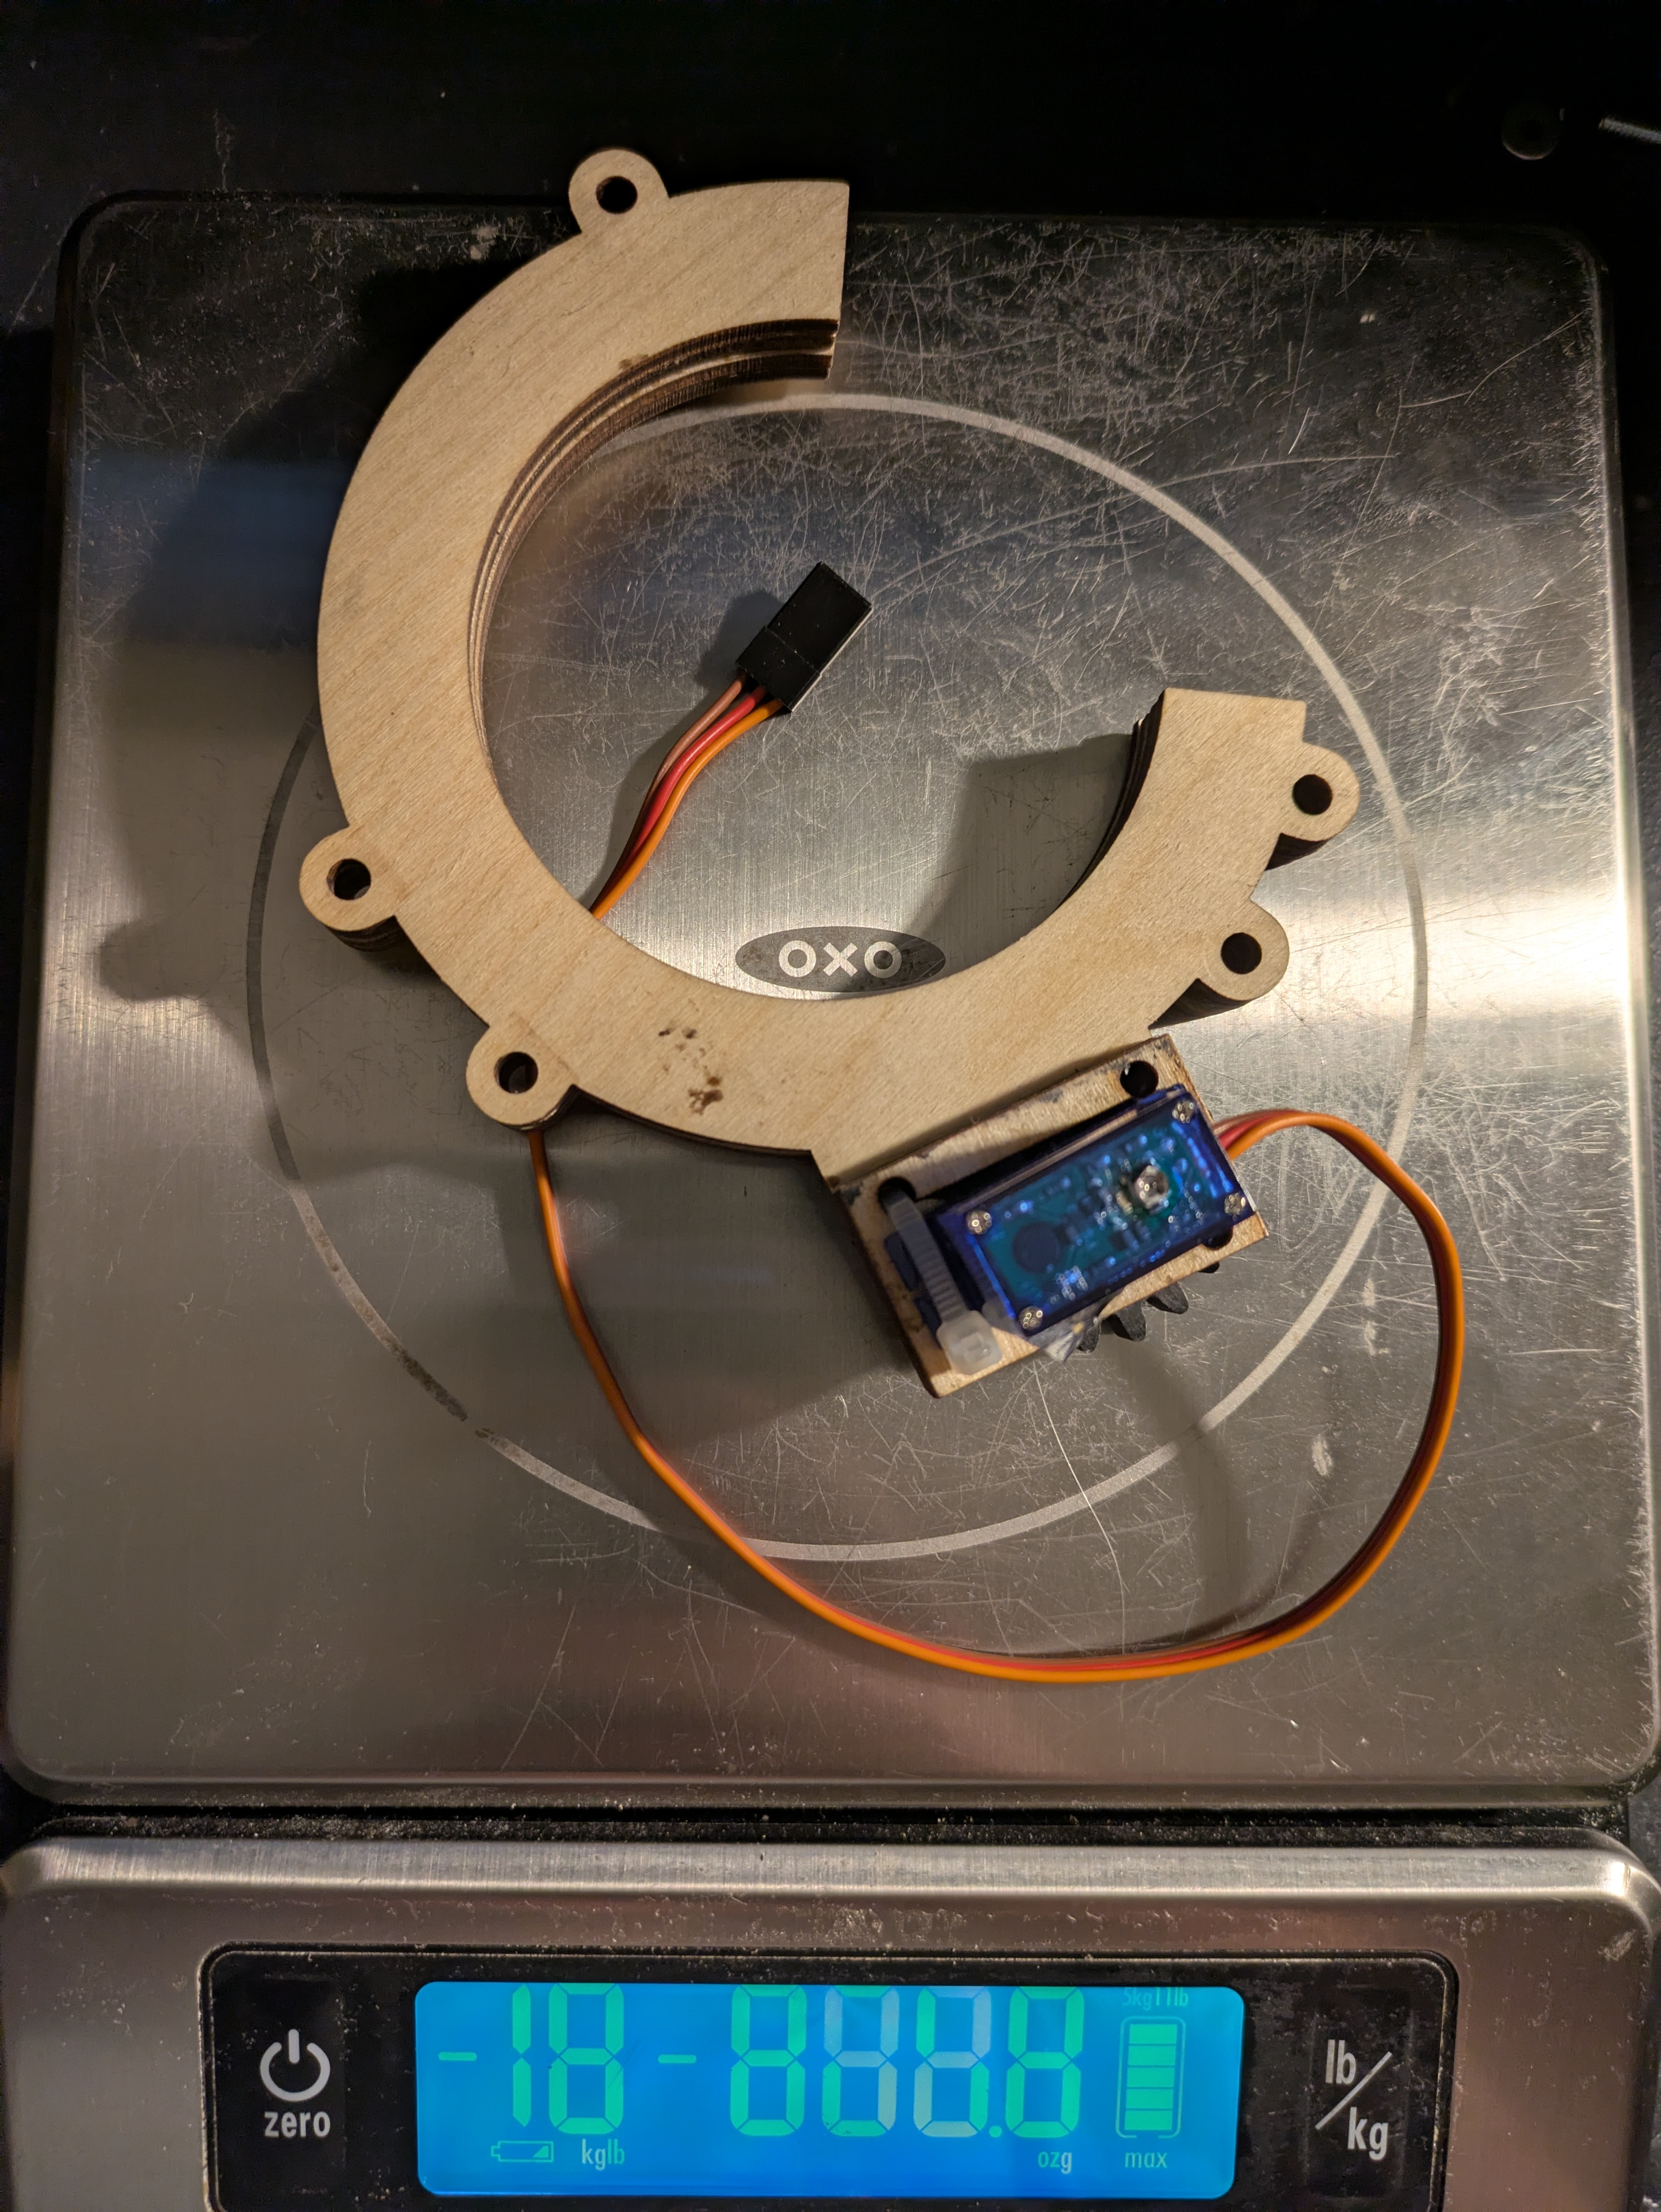
\includegraphics[width=0.2\textwidth]{sections/results/parts-grasper-1.jpg} & 41.5 \\
        CPU, Cameras, and Other Electronics & 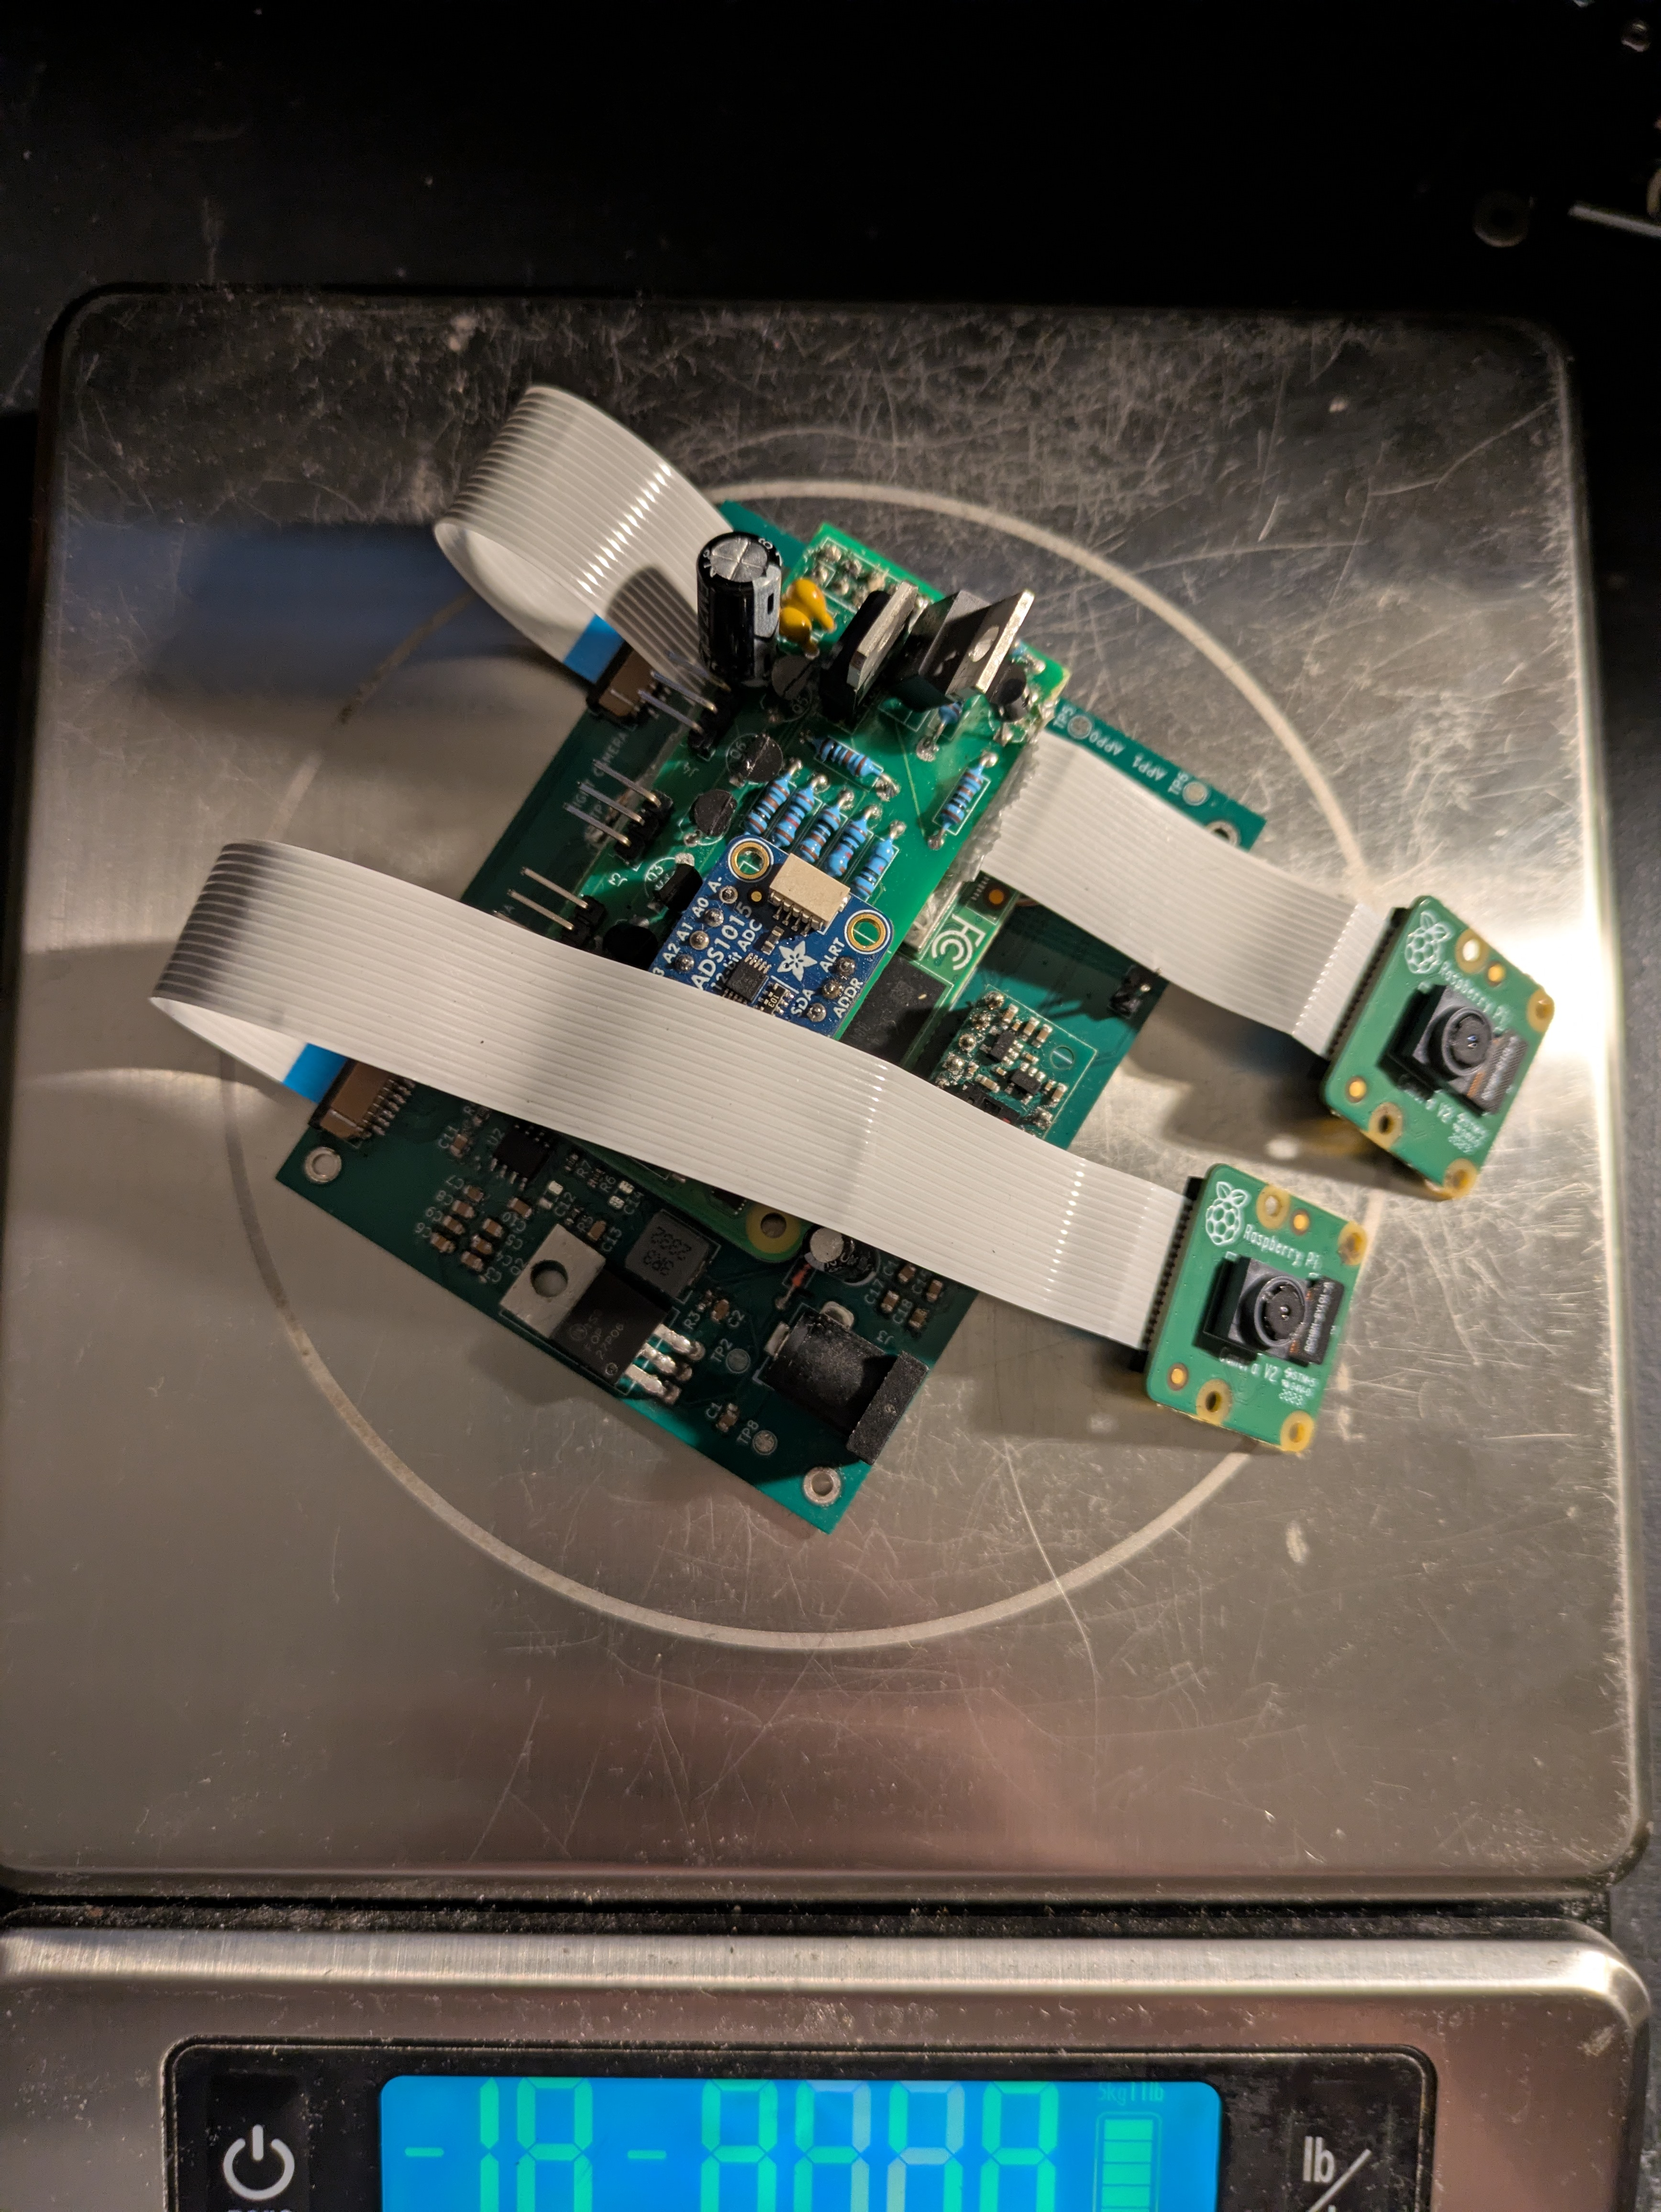
\includegraphics[width=0.2\textwidth]{sections/results/parts-electronics.jpg} & 72 \\
        Nuts and Bolts & 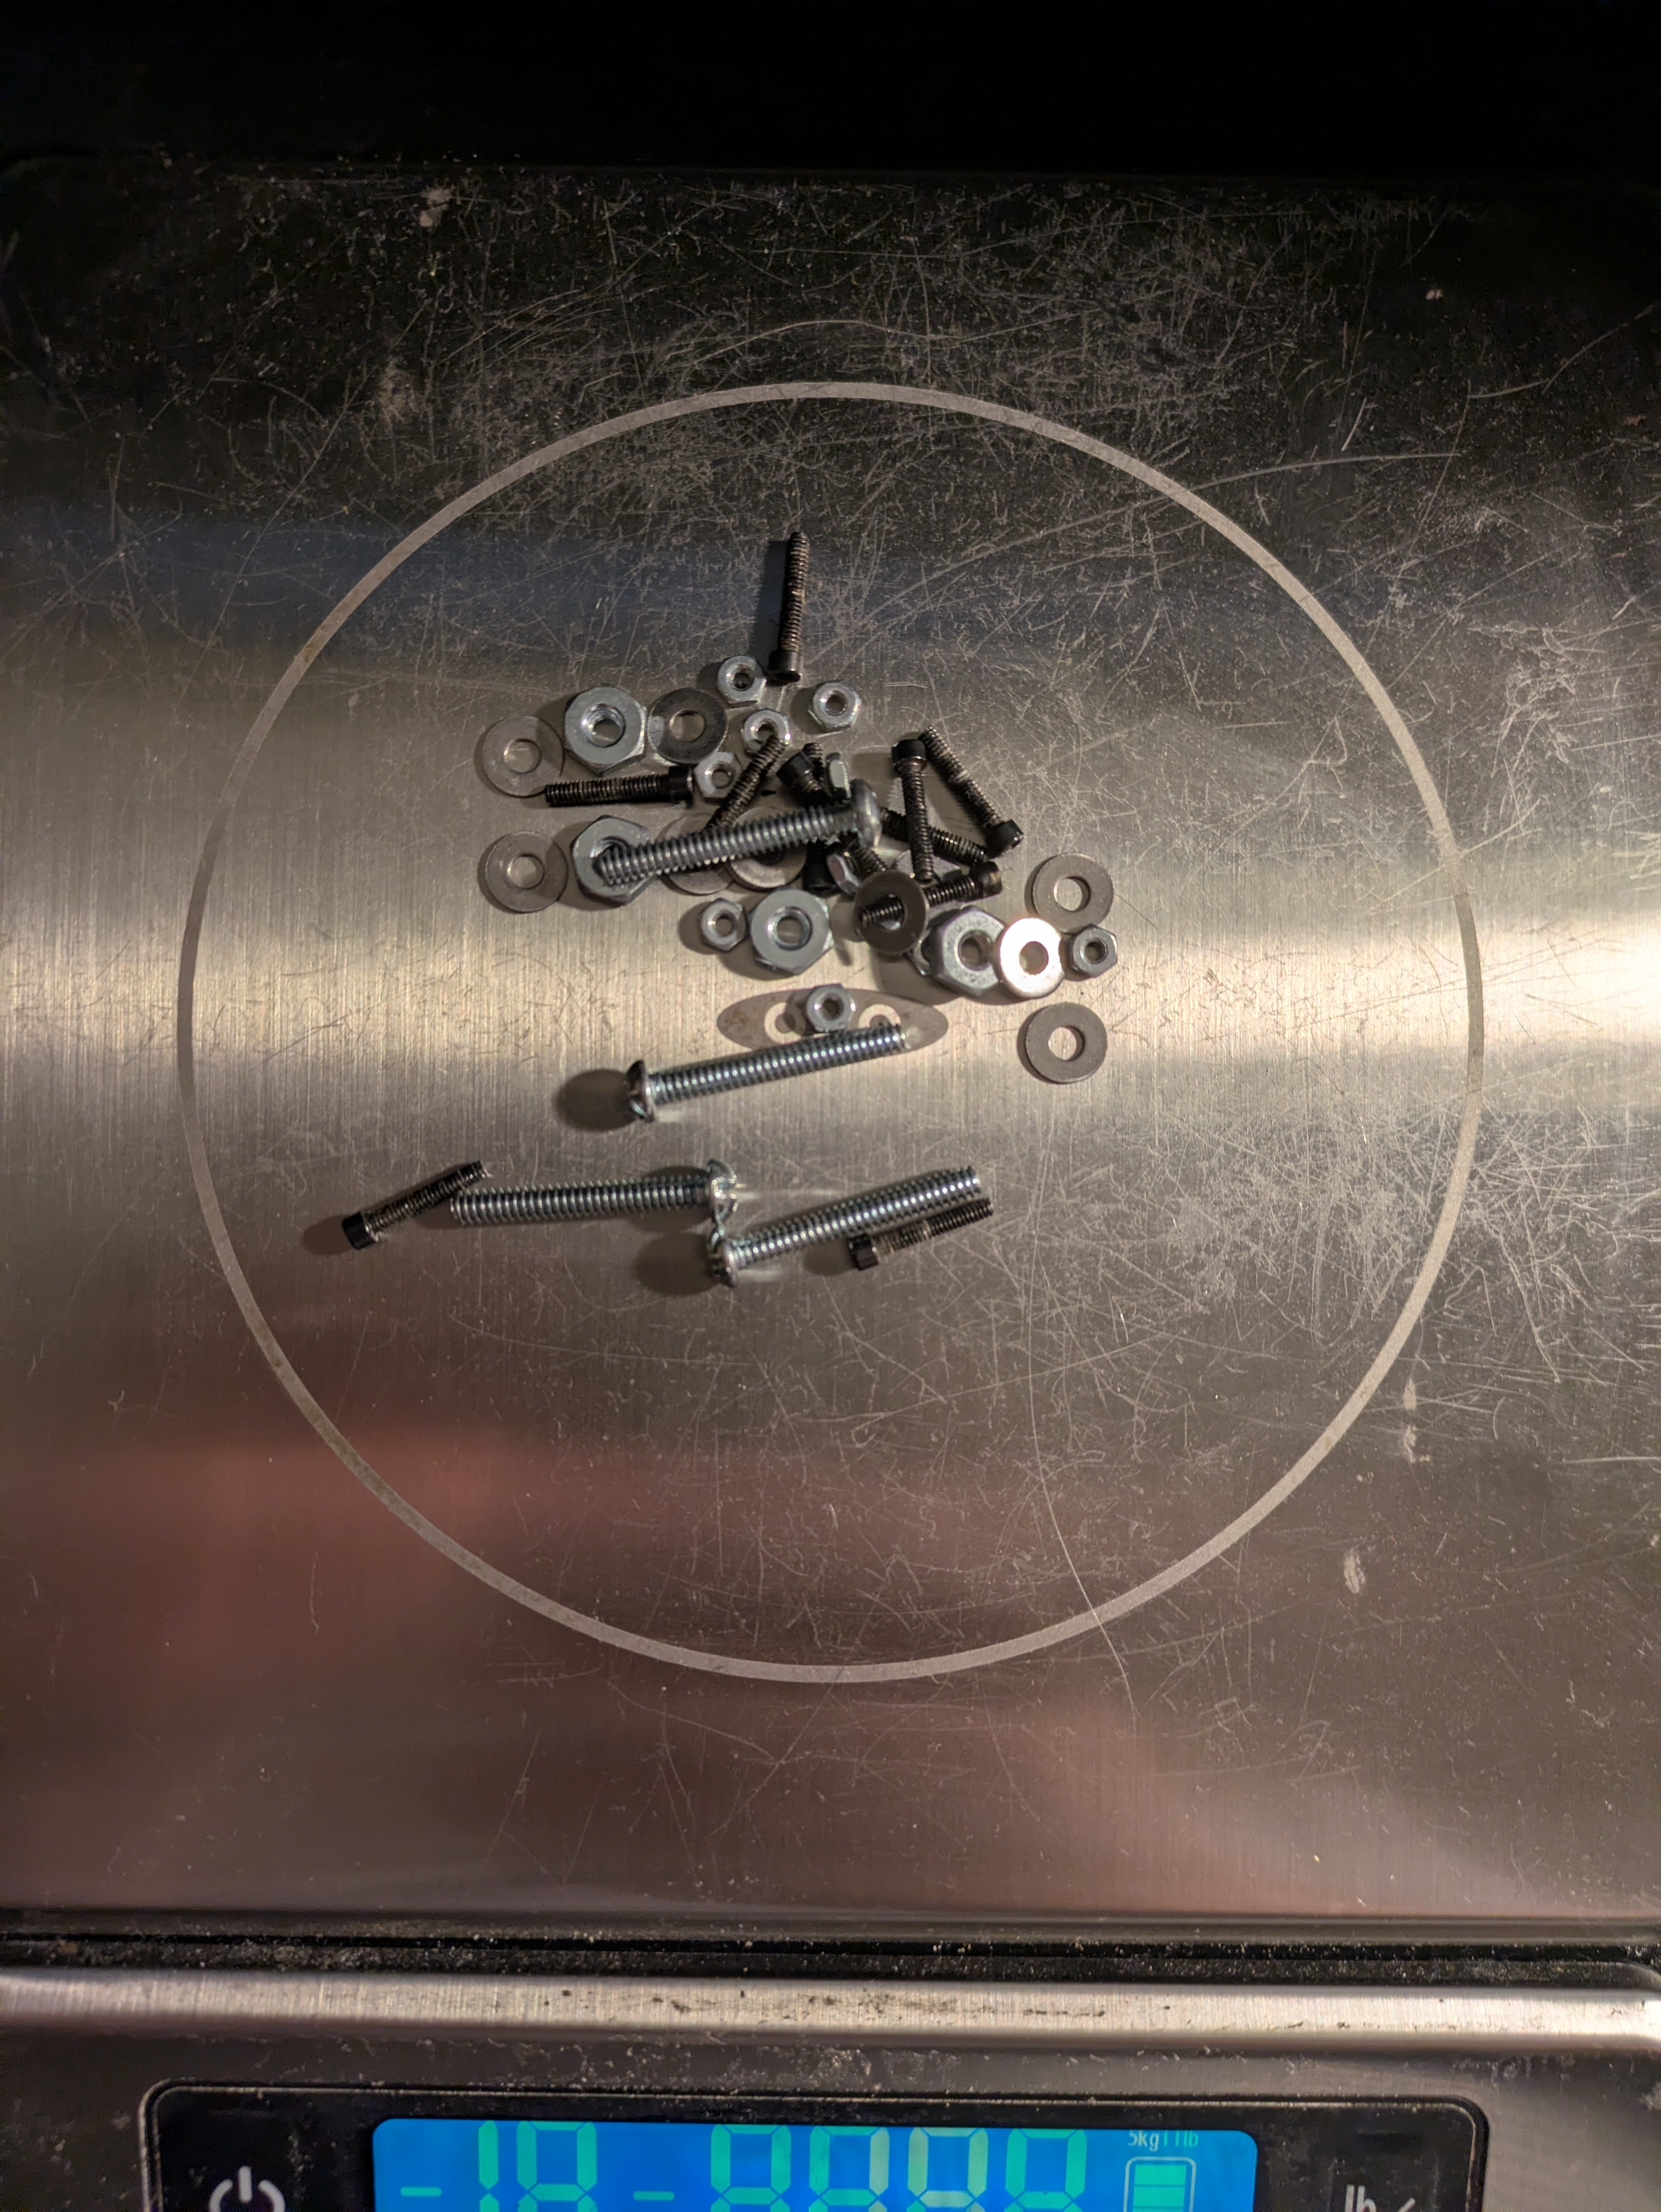
\includegraphics[width=0.2\textwidth]{sections/results/parts-bolts.jpg} & 19 \\
        \hline
        Total Weight & - & 236 \\
        \hline
    \end{tabular}
\end{table}


\subsubsection{Repeatability} \label{sec:results:repeatability}

Of the 30 grasping cycles tested, 6 cycles resulted in a failure to grasp or release successfully,
for an overall success rate of 80\%. Table \ref{tab:grasp-failure} shows the failure cases identified during the test
with a brief explanation of each, and the number of times each failure occurred.

One important detail that is not captured in the tabulated data is that all 4 cases of the "Failure to Detect Released Position"
failure occurred continuously towards the end of the test, from trial 24 to 27. After trial 27 the servos were inspected, and it
was found that the zero point of one had drifted significantly. After retuning its zero point, this failure did not occur for the 
remaining two trials.

\begin{table}[H]
    \centering
    \caption{Grasper Failure Cases and Counts}
    \label{tab:grasp-failure}
    \begin{tabular}{
        |>{\raggedright\arraybackslash}m{0.33\textwidth}|>{\raggedright\arraybackslash}m{0.33\textwidth}||
        >{\raggedright\arraybackslash}m{0.15\textwidth}|}
        \hline
        Failure & Description & Count\\
        \hline
        Premature Current Limit While Grasping & {The current limit used to detect when the grasper has reached its fully closed
        position was triggered before the closed position had actually been reached.} & 2 \\
        Failure to Detect Released Position & {The current limit used to detect when the grasper has reached its fully opened
        position was not triggered within roughly 20 seconds of it reaching the fully opened position.} & 4\\
        \hline
    \end{tabular}
\end{table}
